\section{Date: 2024-10-30}
\noindent \textbf{Series ID: DISC6221ALLEST176QNSA} 

\noindent This series is titled Total Discharges for General Medical and Surgical Hospitals, All Establishments and has a frequency of Quarterly. The units are Thousands of Units and the seasonal adjustment is Not Seasonally Adjusted.The observation start date is 2012-07-01 and the observation end date is 2024-04-01.The popularity of this series is 0. \\ 

\noindent \textbf{Series ID: CES4300000034} 

\noindent This series is titled Indexes of Aggregate Weekly Hours of Production and Nonsupervisory Employees, Transportation and Warehousing and has a frequency of Monthly. The units are Index 2002=100 and the seasonal adjustment is Seasonally Adjusted.The observation start date is 1972-01-01 and the observation end date is 2024-09-01.The popularity of this series is 1. \\ 

\subsection{Regression Tables and Plots}
\begin{center}
\begin{tabular}{lclc}
\toprule
\textbf{Dep. Variable:}                     & value\_fred\_CES4300000034 & \textbf{  R-squared:         } &     0.344   \\
\textbf{Model:}                             &            OLS             & \textbf{  Adj. R-squared:    } &     0.330   \\
\textbf{Method:}                            &       Least Squares        & \textbf{  F-statistic:       } &     24.12   \\
\textbf{Date:}                              &      Wed, 30 Oct 2024      & \textbf{  Prob (F-statistic):} &  1.19e-05   \\
\textbf{Time:}                              &          19:57:57          & \textbf{  Log-Likelihood:    } &   -197.22   \\
\textbf{No. Observations:}                  &               48           & \textbf{  AIC:               } &     398.4   \\
\textbf{Df Residuals:}                      &               46           & \textbf{  BIC:               } &     402.2   \\
\textbf{Df Model:}                          &                1           & \textbf{                     } &             \\
\textbf{Covariance Type:}                   &         nonrobust          & \textbf{                     } &             \\
\bottomrule
\end{tabular}
\begin{tabular}{lcccccc}
                                            & \textbf{coef} & \textbf{std err} & \textbf{t} & \textbf{P$> |$t$|$} & \textbf{[0.025} & \textbf{0.975]}  \\
\midrule
\textbf{const}                              &     380.4686  &       49.588     &     7.673  &         0.000        &      280.653    &      480.284     \\
\textbf{value\_fred\_DISC6221ALLEST176QNSA} &      -0.0273  &        0.006     &    -4.911  &         0.000        &       -0.039    &       -0.016     \\
\bottomrule
\end{tabular}
\begin{tabular}{lclc}
\textbf{Omnibus:}       &  3.469 & \textbf{  Durbin-Watson:     } &    0.481  \\
\textbf{Prob(Omnibus):} &  0.176 & \textbf{  Jarque-Bera (JB):  } &    2.867  \\
\textbf{Skew:}          & -0.598 & \textbf{  Prob(JB):          } &    0.238  \\
\textbf{Kurtosis:}      &  3.041 & \textbf{  Cond. No.          } & 2.04e+05  \\
\bottomrule
\end{tabular}
%\caption{OLS Regression Results}
\end{center}

Notes: \newline
 [1] Standard Errors assume that the covariance matrix of the errors is correctly specified. \newline
 [2] The condition number is large, 2.04e+05. This might indicate that there are \newline
 strong multicollinearity or other numerical problems.

\begin{figure}
\centering
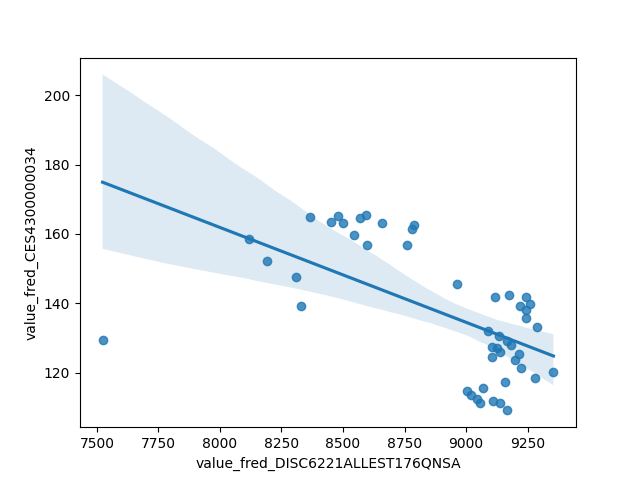
\includegraphics[scale = 0.9]{plots/plot_2024-10-30.png}
\caption{Regression Plot for 2024-10-30}
\end{figure}
\newpage
